\documentclass[12pt]{article}

\usepackage{amssymb,amsthm,amsmath}
\usepackage{mathtools} 
\usepackage{graphicx}
\usepackage{geometry,lscape}
\usepackage{longtable,multirow}
\usepackage{booktabs}
\usepackage{bbold}
\usepackage{chngcntr}

\counterwithout{figure}{section}
\counterwithout{figure}{subsection}
\counterwithout{table}{section}
\counterwithout{table}{subsection}

\newtheorem{assumption}{Assumption}
\newtheorem{proposition}{Proposition}

\setlength{\parindent}{0pt}
\geometry{a4paper}

\newcommand{\E}{\mathbb{E}}
\newcommand{\N}{\mathcal{N}}
\newcommand{\1}{\mathbb{1}}
\DeclareMathOperator{\sign}{sign}
\DeclareMathOperator{\mean}{mean}
\DeclareMathOperator{\var}{var}
\DeclareMathOperator{\sd}{sd}
\DeclareMathOperator{\cov}{cov}
\DeclareMathOperator{\corr}{corr}
\DeclareMathOperator{\Prob}{Prob}

\title{Jobless Recovery and Skill Mismatch}
\date{}
\author{Rong Fan}

\begin{document}
\maketitle
\begin{abstract}
In a business cycle model with search and matching frictions, I explain the slow jobless recovery to be the result of a mismatch between worker skill and firm technology. The mismatch penalty increases the unemployment level and volatility, mainly by increasing the probability of matching failure. The impact of mismatch penalty is more significant when skill variance is higher and when technology is more skill-complementary. The mismatch also decreases the labor force participation rate. 
I extend the model by allowing workers and firms to adjust their skill and technology level. Endogenous skill and technology amplify the mismatch fluctuation, especially when the return to capital is high and the cost of technology adoption is significantly lower than the cost of training. Fewer adjustments are made during the recession, and the matching failure probability is higher during the recession. At the same time, the technology level chosen during the expansion can be too high for the recession and leads to higher matching failure probability due to mismatch penalty. 
Using state-level data, I find that mismatch is vital in explaining the state variation of the unemployment rate and volatility. 
By calibrating the full model to match the 1980-1986 and 2007-2013 data, I find an increased mismatch level in 2007-2013. The higher mismatch level is mainly attributed to a higher complementarity between skill and technology, higher skill variance, and lower technology adoption cost. 
Compared with the allocation selected by the social planner, the agents fail to internalize the value of future matches and their impact on the labor market condition. The decentralized market creates too many vacancies, has too high an unemployment exit rate, and invests too little in training. Higher unemployment insurance can increase the matching quality and decrease vacancy creation. Subsidies to training can decrease the mismatch by increasing the investment in training. 

\end{abstract}

\clearpage
\section{Introduction}
The recovery from the Great Recession has been accompanied by the unemployment rate remaining stubbornly high for extended periods, with a higher proportion of long-term unemployed. After peaking at 10\% in October 2009 (almost 40\% are long-term unemployed), the unemployment rate remained above its pre-recession level until November 2016. Right before the pandemic, the unemployment rate had recovered, and in fact, reached 3.5\% in February 2020, which is the lowest level since 1969. However, the Labor Force Participation Rate (LFPR) remained at a much lower rate (63.3\% in February 2020) than the pre-recession level  (66\% in November 2007).\footnote{data source: FRED} \\

There was substantial heterogeneity in employment recovery paths across education groups in the 2001 and 2008 recession. The employment of low-skill workers (high school or less) dropped significantly during the Great Recession and much steeper than in the 2001 recession. Also, unlike the quick recovery in the 2001 recession, the employment of low-skilled workers stayed significantly below its pre-recession level after the 2008 recession (9 million compared with 11.5 million).  In terms of the high skilled workers (some college, bachelor's, and higher), the effect of recessions on employment was limited, followed by a quick recovery. 

In this paper, I develop a theoretical framework to conceptualize the notion of skill-technology mismatch and apply this to uncover the underlying sources of the jobless recovery after the great recession. This theory is qualitatively consistent with three features of the Great Recession: (1) excessive response and slow recovery of unemployment rate and labor force participation rate; (2) decline trend of labor force participation rate; (3) heterogeneous recovery path of different skill group. \\

This model is an extension of Moscarini and Postel-Vinay (2018)\cite{MPV2018}, where they propose a business cycle model with random job search both off- and on-the-job (OJS). Matches are heterogeneous in productivity, drawn randomly from a 
cumulative distribution function $\Gamma$ after the match is formed. The wage is determined by Bertrand-competition as in the Sequential Auctions protocol of Postel-Vinay et al.(2002)\cite{PostelVinayetal2002}, so the value function is independent of the state variable, and the model is highly tractable. I extend the model in two ways: firstly, instead of having the match quality be a random draw from an exogenous distribution, the match quality in this paper is endogenous and determined jointly by the worker's skill level and the firm's technology level; secondly, workers receive home productivity shocks and faces labor force participation decision. In the baseline model, the skill level is drawn from a cdf $\Gamma_a$ when workers enter the labor market; technology level is drawn from a cdf $\Gamma_b$, and is revealed only after the firm get matched to a worker successfully. Home productivity is drawn from a cdf $\Gamma_n$ each period, and workers make the labor force participation decision every period.  \\

To model the mismatch, I adopted the framework of Lise and Postel-Vinay(2020)\cite{LisePV2020}, the surplus of the match is increasing in the skill and technology level in general, but it also receives a mismatch penalty due to over-qualification (worker receives extra disutility due to his overly high skill level) or under-qualification (worker is not qualified enough for the task). \\

The expected output of the match is increasing in the aggregate skill and technology level but decreasing in the gap between skill and technology. The importance of mismatch depends on the skill distribution and the complementarity level between skill and technology. When keeping the average skill level the same, higher skill dispersion increases the expected mismatch penalty received by the firm and the probability of matching failure. When the skill and technology are more complementary, the mismatch becomes more costly, and the skill-technology difference affects more the match surplus. \\

The mismatch affects the unemployment rate through frictional unemployment (job finding rate) and mismatch unemployment (unsuccessful match due to mismatch penalty). The mismatch penalty lowers the vacancy value, which decreases the job creation incentives and job finding rate. It takes longer for the workers to get matched, and the frictional unemployment rate is increased. The mismatch penalty also makes some matches' surplus negative; workers who get matched will reject the offer and stay unemployed. The mismatch unemployment will depend on the probability of match surplus being negative. \\

In a standard DMP model, the job arriving rate responds to the labor productivity shock through free entry conditions. The mismatch penalty dampens the job arriving rate volatility. The response of vacancy value to Total Factor Productivity (TFP) is smaller when there is a mismatch penalty. When TFP is higher, more matches will receive a mismatch penalty (extensive margin), and the average mismatch penalty received is higher (intensive margin). At the same time, when the unemployment rate is lower, the firms are more likely to get matched with low-skilled workers, and the matches are more likely to fail. The mismatch penalty increases unemployment volatility mainly through the mismatch unemployment fluctuation. The probability of matching failure decreases in TFP. The response is asymmetric; the mismatch unemployment responds more to a negative TFP shock. \\

The mismatch also decreases the labor force participation rate. The workers are more likely to leave the labor force when the mismatch penalty lowers the expected value of staying in the labor force. The labor force participation rate is pro-cyclical; more workers leave the labor force during the recession because the more matches have surplus lower than the home production. \\

I extend the model by allowing workers and firms to adjust their skill and technology levels. To endogenize the training and technology adoption decision, I mainly use the framework in Stokey(2014)\cite{Stokey2014}, but without the growth and stochastic component. Heterogeneous firms and workers adjust their skill or technology level by paying an adjustment cost convex in the change. The model also captures the dynamics of workers and firms. 
The human capital dynamics are following Stantcheva(2015)\cite{Stantcheva2015}, workers acquire their human capital through learning-or-doing and are facing ability shocks; the human capital depreciates if the worker is unemployed or out of labor force. 
The firm dynamics are similar with Luttmer(2012)\cite{Luttmer2012}, where incumbents are facing permanent productivity shocks and will leave the market if the productivity is lower than a certain threshold.  \\

When the training and technology adoption decisions are endogenous, agents invest in human capital and technology to maximize their gain. Training and R\&D investment are pro-cyclical; during expansion, more workers will get matched with the firms, and out of all the new matches, more workers and firms will choose to upgrade their skill and technology (extensive margin), and each worker and firm will invest more (intensive margin). The skill and technology adjustment allows more matches to be successful during the expansion since the productivity gain from adjustment is higher when the productivity is high. \\


The optimal skill and technology level picked by the matched worker and firm does not necessarily minimize the level of mismatch. The upgrade decision made during the expansion could make the match more vulnerable during the recession. During the expansion, the productivity gain is more significant, so the firms choose to upgrade their technology level to maximize the match surplus. However, during the recession, the productivity gain becomes smaller, while the mismatch penalty becomes more significant. The endogenous skill and technology cause more mismatch during the recession when technology adoption cost is significantly lower than training cost. Suppose firms can benefit by upgrading their technology at a low cost. In that case, they will choose a high technology level even though it causes a higher mismatch in the future.  \\

I compare the decentralized equilibrium with the social planner's problem. In addition to the externalities related to match frictions, an additional externality, mismatch externality, arises. The agents fail to internalize their impact on the labor market condition and the value of future matches. A lower unemployment rate increases the probability of matching failure and decreases the payoff of an additional vacancy creation. The decentralized market creates too many vacancies and has too high an unemployment exit rate.  \\

In the decentralized market, the agents underinvest in their training because they fail to internalize the value of future matches. For the employed workers, they invest in their training to maximize the output of the current match. However, they fail to internalize the future social value if they get separated from the firm. The unemployed workers do not invest in their training since it has no impact on their wage contract value and fails to internalize their social value. \\


The full model is calibrated to match the data from 1980-1986 and 2007-2013, respectively. I use the Macro Data moments (unemployment rate, job-to-job transition, etc.) and the Micro Data moments (wage dynamics). By comparing the calibration result, the mismatch level is higher in 2007-2013 than in 1980-1986. The higher mismatch level is mainly attributed to a higher skill variance, a higher skill-technology complementarity, and a lower technology adoption cost.  \\

Higher unemployment insurance can decrease the inefficiency caused by the mismatch. Higher unemployment insurance encourages labor force participation and increases the employment level even though the unemployment rate is higher.  Also, workers are more patient and only accept better matches, the match output is higher, and each match can last longer.  The subsidies to training investment decrease the level of mismatch. More investments are made in training; workers are less likely to leave the labor force when they get unemployed with a higher skill level.  \\

I use the state-level data to test the main analytical results. I use education (share of the population with bachelor's or higher) as an approximation of skill level, and the number of patents claimed in the state as an approximation of technology level. All the measures are normalized as deviation from the national average to make skill and technology levels comparable. While controlling the state fixed effect and national unemployment trend, I find that unemployment rate and volatility decrease in skill and technology level, but increases in the skill-technology difference.  \\

This paper is related to studies on the unemployment rate and the labor force participation rate after the Great Recession. 
Firstly, the Great Recession had a heterogeneous impact on different demographic groups. 
Mattingly et al.(2011)\cite{Mattinglyetal2011} found that the recession mainly affects men, single parents, young adults, and people with less education;
Zhang et al.(2015)\cite{Zhangetal2015} find that the unemployment rate varied with the level of education; 
Charles(2016)\cite{Charles2016} found that the decline concentrated in low-skilled workers, accompanied with an increase of transitions from employed to not in the labor force (Frazis 2017\cite{Frazis2017}). 
My paper provides a theoretical framework to explain the empirical findings on group heterogeneity.   \\

Secondly, the low employment during the Great Recession is not only cyclical but also structural. 
Pissarides(2013)\cite{Pissarides2013} provided evidence that the USA suffered from structural unemployment during the recovery;
Estev{\~a}o and Tsounta(2011)\cite{EstevaoTsounta2011} presented econometric evidence that the recession increases structural unemployment mainly through skill mismatches and housing market performance;
Furlanetto and Groshenny(2016)\cite{FurlanettoGroshenny2016} included mismatch shocks in their model, and found they are only important during the recession;
Van Zandweghe(2012)\cite{VanZandweghe2012} argued that the trend component is essential to understand the decline in labor force participation rate;
while Aaronsonetal(2014)\cite{Aaronsonetal2014} provided evidence that population aging can only explain at most half of the trend decline;
Yagan(2019)\cite{Yagan2019} argued that the decline of labor force participation rate is imposed by the Great Recession.
My model's prediction is consistent with the empirical findings; the types of matches on the labor market during the recession are different from those during the expansion.  \\

This paper is strictly related to skill mismatch literature. There is a growing literature based on skill mismatch in recent years, focusing more on the skills used in work instead of just education level. Desjardins and Rubenson(2011)\cite{DesjardinsRubenson2011} analyzed skill mismatch using direct measures of skills based on the 2003-2007 Adult Literacy and Lifeskills Survey (ALLS), and found that 30\%-40\% workers are over- or under-qualified. McGowana and Andrews(2015)\cite{McGowanAndrews2015} find a negative relationship between mismatch and labor productivity using the Survey of Adult Skills (PIAAC). B{\"o}hm et al.(2020)\cite{Bohmetal2020} found that return to skills differs across employers, which affects the earnings. 
Lise and Postel-Vinay(2020)\cite{LisePV2020} and Guvenen et al.(2020)\cite{Guvenenetal2020} developed empirical measures of multidimensional skill mismatch and focus on the wage pattern of the workers, using the 1979 National Longitudinal Survey of Youth (NLSY79) combined with occupation-level data on skill requirements from the O*NET. Instead of examining the impact of skill mismatch on worker's earning, my paper focuses more on the impact on employment level.  
The most relevant paper is Restrepo (2015)\cite{Restrepo2015}, which focused on structural unemployment and extended the search and matching model to include several types of jobs and workers. I introduce richer and continuous heterogeneity into the model and discuss the interaction between the recession and the mismatch. \\

The paper is organized as follows. Section 2 introduces the baseline model. Section 3 and 4 discuss the analytical results. Section 5 lays out the formal model and the estimation results. Section 6 presents empirical evidence. Section 7 concludes the paper. 

\section{Search Model with heterogeneous firms and workers}
In this section, I build a business cycle model with search and matching frictions in the labor market and labor force participation choice, in which the match quality is decided jointly by the worker's skill and the firm's technology. 

\subsection{Environment}
Time $T = 1, 2, 3 \dots$ is discrete and continues forever; the economy is populated by a continuum of risk-neutral workers with measure 1. Both workers and firms maximize their present value of income or profit, with a discount rate $\beta$. Firms produce a single, homogeneous, nonstorable numeraire consumption good, using only labor. \\

\textbf{Production function: }
The production function is a function of aggregate productivity ($z$), labor skill ($a$), and firm's technology level ($b$). $z$ is common to all matches, and $\log z$ evolves according to an AR(1) process with persistency $\rho_z$. 
\begin{align*}
\log z' = \rho_z \log z +\epsilon_z
\end{align*}
The production increases in $z$, $a$, and $b$, but there is a penalty associated with the skill mismatch. If the worker is under-qualified ($a<b$), the firm receives a mismatch penalty $\alpha_u(b-a)^2/b$ because the worker is not qualified enough to complete all the tasks required by the firm. If the worker is over-qualified ($a<b$), the worker receives an extra disutility $\alpha_o(a-b)^2/a$. $\alpha_u$ and $\alpha_o$ measure the magnitude of productivity penalty and disutility when skill and technology are mismatched.  \\

\textbf{Worker: }
Workers are heterogeneous in terms of their skill level $a_i$; they get their initial skill level from the distribution $\Gamma_a$. 
When the worker is unemployed, his human capital depreciates at rate $\delta_a$. \\

Each worker receives an idiosyncratic home production shock at the beginning of each period, noted by $\epsilon_n$, and drawn from Pareto distribution $\Gamma_n$. The unemployed worker receives unemployment leisure $b_u$ if he stays in the labor force. The employed worker receives wage $\omega(z,a,b',b)$ (explained later) if he stays in the labor force. The worker who chooses to leave the labor market receives the home production $\epsilon_n$. If the worker leaves the labor force, he will not be matched to any firms during the period. He will be automatically unemployed next period. 

\begin{align*}
\epsilon_n &\sim Pareto(\epsilon_{min},\lambda_n)  \\
\E\epsilon_n &= \frac{\lambda_n}{\lambda_n-1}\epsilon_{min}
\end{align*}

\textbf{Firm: }
Firms are heterogeneous in terms of their technology level $b_j$. 
When firms firstly enter the market, they get their initial technology type from the distribution $\Gamma_b$. 
When the match is newly formed, firms can train the worker and upgrade their technology level by paying an adjustment cost to maximize the profit. 
After entering the market, the technology level of the firm depreciates at a rate $\delta_b$. \\

\subsection{Search and Match}
The match is random. All the unemployed workers $u$ and share $s$ of the employed workers $e$ are searching. With probability $\delta$, the match is destroyed exogenously, so the number of employed workers searching for a new job is $s(1-\delta)e$. Firms pay a fixed cost of $c$ to create and advertise the vacancy each period. 
The effective job market tightness $\theta$ is the ratio between vacancies $\nu$ and workers actively searching of the job $u+s(1-\delta)e$. 
\begin{align*}
\theta = \frac{\nu}{u+s(1-\delta)e}
\end{align*}
The matching function is assumed to be Cobb-Douglas, the job arriving rate $\phi$ is a function of the market tightness.  
\begin{align*}
\phi_t(\theta) = \Phi \theta_t^\alpha
\end{align*}

\subsection{Value of not-in-labor-force, unemployment and employment }
The value of not in the labor force is $V_n(\epsilon_n)$ depending on the home productivity received by the worker; the value of unemployment is constant $V_u$ for all the workers. The expected value of the match's total output is noted as $P(z,a,b)$; $D(z,a,b)$ represents the expected value of over-qualification disutility; the net surplus of the match is noted as $S(z,a,b)$, which is $P(z,a,b)$ subtracted by $V_u$ (opportunity cost) and $D(z,a,b)$ (disutility). The value of employment (contract) is $V_e(z,a,b',b)$, which depends not only on TFP $z$, worker's skill level $a$ and firm's technology level $b$, but also his most recent employment history $b'$, which determines his bargaining power. 

\subsection{Wage determination}
The wage is determined by Bertrand competition; workers accumulate bargaining power during employment. When firstly enter the labor market, workers do not have any bargaining power. The value of the contract will only be $V_u+D(z,a,b)$, since it is the minimum contract the firm needs to promise to have the worker accept the job. If the worker is not over-qualified ($a \leq b$), the contract value would be the same as the value of unemployment $V_u$. If the worker is over-qualified ($a>b$), the wage payment needs to be $V_u+D(z,a,b)$, since the firm needs to compensate the extra disutility.  

\begin{table}[h!]
\centering
\begin{tabular}{llc}
\hline \hline
New match Surplus & Contract  \\
\hline
$S(z,a,b) \leq 0$ &Stay unemployed \\
$S(z,a,b)>0$ &$V_e(z,a,0,b) = V_u+D(z,a,b)$ \\
\hline \hline
\end{tabular}
\caption{Wage for unemployed workers}
\label{Wage_UE}
\end{table}

As workers search on the job and meet new employers, they start to gain bargaining power, since the new and old employers need to compete over the workers. Consider a worker with current wage contract $V(z,a,b'',b)$. With probability $s\phi(\theta_t)$, he meets a new employer with technology level $b'$. If the new match can generate higher surplus $S(z,a,b')>S(z,a,b)$, in order to win the auction, the new employee needs to promise at least how much the old employee is able to deliver, which is $S(z,a,b)$. Then the worker will choose to jump to the new match, and the value of new contract is $V_e(z,a,b,b') - D(z,a,b') = S(z,a,b)$, the bargaining power is increased to $S(z,a,b)/S(z,a,b')$. If the new match generates lower surplus $S(z,a,b')\leq S(z,a,b)$, then there are 2 cases. If the maximum value the new match can deliver to the worker is less than the worker's current contract value $S(z,a,b') \leq V_e(z,a,b'',b)-D(z,a,b'')$, then nothing would change; otherwise, the old employee will pay at least how much the new employee is able to afford to keep the worker. The worker will stay at the old job with a promotion, the value of contract will increase to $P(z,a,b')$, and the bargaining power will increase  to $S(z,a,b')/S(z,a,b)$. 

\begin{table}[h!]
\centering
\begin{tabular}{ll}
\hline \hline
New match Surplus & Contract  \\
\hline
$S(z,a,b') \leq V_e(z,a,b'',b)-D(z,a,b)$  &  \multirow{2}{*}{$V_e(z,a,b'',b)=S(z,a,b'')+D(z,a,b)$} \\
\text{and } $S(z,a,b') \leq S(z,a,b)$ & \\
$S(z,a,b') > V_e(z,a,b'',b)-D(z,a,b)$   & \multirow{2}{*}{$V_e(z,a,b',b)=S(z,a,b')+D(z,a,b)$} \\
\text{and } $S(z,a,b') \leq S(z,a,b)$ & \\
$S(z,a,b')>S(z,a,b)$ & $V_e(z,a,b,b')=S(z,a,b)+D(z,a,b')$  \\
\hline \hline
\end{tabular}
\caption{Wage for employed workers}
\label{Wage_EE}
\end{table}

If the worker get separated endogenously or exogenously from the job, the worker lose all the bargaining power, and will have to start to climb on the wage ladder again. \\



\subsection{Timing of Events}
\begin{enumerate}
\item Nature draws the $\epsilon_t$ innovation to TFP $z_t \sim AR(1)$, and firms and workers observe the realization of the productivity shock. 
\item Idiosyncratic shocks are realized on firms' technology and workers' human capital. 
\item Idiosyncratic shocks on home production are realized, both employed and unemployed decide if they want to stay or leave the labor force.
\item Human capital of unemployed workers depreciates. Technology depreciates. 
\item Existing matches break up: firstly by endogenous separation if the firms or workers can be better off by destroying the match, secondly by exogenous separation with probability $\delta$. When the workers get separated from the firms, they can not search during the current period; they will be part of the unemployed workers and start to search starting from the next period. 
\item Firms and workers produce. Firms pay the workers wage $\omega(z,a,b',b)$ according to their state-contingent contract. Unemployed workers receive the utility from leisure $b_u$. Agents not in the LF receive the home production output. 
\item Firms enter the market and make the vacancy posting decision. When they enter the market, they pay the cost associated with vacancy creation and posting and initial technology adoption. They do not know their type $b$; they only know the distribution of $b$ from which they will draw their type. Firms can observe perfectly the distribution of workers while making the decision. 
\item Firms are randomly matched to previously unemployed workers and a share $s$ of the skill employed workers. At the same time, the firm type $b$ is revealed. 
\item Upon meet, firms offer the contract to their matched workers. If the worker is unemployed, the firm will offer a take-it-or-leave-it contract; if the worker is already employed, his current employee and the new matched firm, while they can observe each others' type perfectly, will Bertrand-compete in the contract. 
\item Unemployed worker will decide to take the contract or not, while employed worker will decide which contract to take. 
\item After the match is successfully formed, workers and firms have the opportunity to increase their skill and technology level by paying an adjustment cost. 
\end{enumerate}

\section{Baseline Model: Exogenous skill and technology}
In the baseline model, I consider the case where the skill and technology are drawn from the distribution. Skill and technology does not depreciate: $\delta_a = \delta_b = 0$. Cost of training and technology adjustment are infinity: $\phi_a \to \infty$ and $\phi_b \to \infty$. There is no on-the-job search $s=0$  \\

Workers are heterogeneous in terms of their skill level $a_i$, they get their initial skill level from skill distribution. 
\begin{align*}
a \sim Pareto(H,\lambda_a)
\end{align*}
Firms are heterogeneous in terms of their technology level $b_j$. When they enter the market, their technology type is unknown. Their type will be revealed after they pay the vacancy cost and enter the market, drawn from the initial distribution. 
\begin{align*}
b &\sim Pareto(Q,\lambda_b)
\end{align*}

\subsection{Value function}
For an unemployed worker, when he is matched to a firm, the firm will only promise to deliver a minimum value $V_{u,t}$ to make the worker indifferent between staying unemployed and taking the job. The value of being unemployed is independent of time and state. The worker always has the choice to leave the LF and get $V_{n,t}(\epsilon_n)$ depending on the shock realized, since the shocks are iid distributed, both $V_n(\epsilon_n)$ and $V_u$ are state independent. 
\begin{align*}
V_{u,t} &= b_u+\beta\E_t\max\{V_{u,t+1},V_{n,t+1}(\epsilon_n)\} = V_u \\
V_{n,t}(\epsilon_n) &= \epsilon_n+\beta\E_t\max\{V_{u,t+1},V_{n,t+1}(\epsilon_n)\} = V_{n}(\epsilon_n) 
\end{align*}
We can drop the time index and solve $V_u$ and $V_n(\epsilon_n)$: 
\begin{align*}
V_u &= b_u+\beta\E\max\{V_u,V_n(\epsilon_n)\} \\
V_n(\epsilon_n) &= \epsilon_n+\beta\E\max\{V_u,V_n(\epsilon_n)\}  \\
\max\{V_u,V_n(\epsilon_n)\} &= \max \{b_u,\epsilon_n\}+\beta\E\max\{V_u,V_n(\epsilon_n)\}  \\
\E\max\{V_u,V_n(\epsilon_n)\} &= \E\max \{b_u,\epsilon_n\}+\beta\E\max\{V_u,V_n(\epsilon_n)\}  \\
\E\max\{V_u,V_n(\epsilon_n)\} &= \frac{1}{1-\beta}\E\max \{b_u,\epsilon_n\}  \\
\E\max \{b_u,\epsilon_n\}  &= b_u+\frac{1}{\lambda_n-1}\epsilon_{min}^{\lambda_n}b_u^{1-\lambda_n} \\
V_u &= b_u+\frac{\beta}{1-\beta}\frac{1}{\lambda_n-1}\epsilon_{min}^{\lambda_n}b_u^{1-\lambda_n} \\
V_n(\epsilon_n) &= \epsilon_n+\frac{\beta}{1-\beta}\frac{1}{\lambda_n-1}\epsilon_{min}^{\lambda_n}b_u^{1-\lambda_n} 
\end{align*}
$V_u$ and $V_n(\epsilon_n)$ are linear in $b_u$ and $\epsilon_n$, the unemployed worker will leave the labor force when $\epsilon_n>b_u$, with probability $\epsilon_{min}^{\lambda_n}b_u^{-\lambda_n}$. To have unemployment rate greater than zero, we need to assume that $\epsilon_{min}<b_u$, so that not all unemployed workers will leave the labor force. The transition probability from unemployed to not-in-the-labor-force $P_{UN}$ is increasing in $\epsilon_{min}$ and decreasing in $\lambda_n$. \\

Output of the match $f(z,a,b)$ is a function of aggregate productivity, worker's skill level, and firm's technology level. It is the net output $g(z,a,b)$ minus the mismatch penalty $p(a,b)$ if the worker is underqualified. If the worker is overqualified, he will receive a disutility $d(a,b)$. The mismatch penalty and disutility could be interpreted as the level of specialization or skill-technology complementarity. The level of complementarity is higher when $\alpha_u$ and $\alpha_o$ are higher.
\begin{align*}
f(z,a,b) &= g(z,a,b)-p(a,b) \\
g(z,a,b) &= z(\kappa a+(1-\kappa) b)\\
p(a,b) &= 1\{a<b\}\alpha_u\frac{(b-a)^2}{b} \\
d(a,b) &= 1\{a>b\}\alpha_o\frac{(b-a)^2}{a}
\end{align*}

The total surplus $S(z,a,b)$, the expected net output $P(z,a,b)$ and the expected disutility $D(z,a,b)$ of the match could be solved as: 
\begin{align*}
S(z,a,b) &= f(z,a,b)-d(a,b)-b_u \\
			 &+(1-\delta)\beta \E_{z'|z}\max\{\E_{\epsilon_n}\max\{S(z',a,b)+b_u,\epsilon_n\}-\E_{\epsilon_n}\max\{b_u,\epsilon_n\},0 \}  \\
D(z,a,b) &=V_u+d(a,b)+(1-\delta)\beta \E_{z'|z}\E_{\epsilon_n}(D(z',a,b)-V_u)1\{{S(z',a,b)+b_u>\max\{b_u,\epsilon_n\}}\} \\
P(z,a,b) &= S(z,a,b)+D(z,a,b)
\end{align*}

In order to solve the total surplus, we need to solve $\E_{\epsilon_n}\max\{S(z,a,b),\epsilon_n\}$ and $\E_{\epsilon_n}\max\{V_u,V_n(\epsilon_n)\}$. Notice that the employed worker will leave the labor force if he receives home production shock $\epsilon_n>\epsilon^*(z,a,b)$, while $\epsilon^*(z,a,b) = S(z,a,b)+b_u$. 
\begin{align*}
&\max\{\E\max\{S(z,a,b)+b_u,\epsilon_n\}-\E\max\{b_u,\epsilon_n\},0 \}   \\
&= \begin{dcases}
0 & ,S(z,a,b) < b_u \\
S(z,a,b) +\frac{1}{\lambda_n-1}\epsilon_{min}^{\lambda_n}((S(z,a,b)+b_u)^{1-\lambda_n}-b_u^{1-\lambda_n}) & ,S(z,a,b)\geq b_u 
\end{dcases}
\end{align*}	

The match surplus as a function of output with different $\lambda$ is plotted in figure \ref{Analytical1}. With different $\lambda$, the decision rule for accepting the job is the same; the unemployed worker will accept and keep the job when $S(z,a,b)>0$. While keeping the expected value of $\epsilon_n$ the same, with higher $\lambda_n$, the workers have fewer outside options. The match surplus function is steeper, and the inequality between matches is greater. The employed worker will leave the labor force if $\epsilon_n>S(z,a,b)+b_u$, and the probability is $(\epsilon_{min}/(S(z,a,b)+b_u))^{\lambda_n}$.  While keeping the expected value of $\epsilon_n$ the same, with higher $\lambda_n$, this probability of leaving the labor force is smaller. \\
\begin{figure}[h!]
\centering
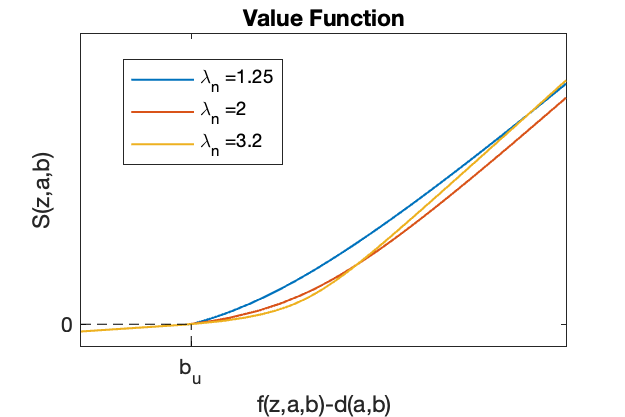
\includegraphics[width=0.48\textwidth]{Analytical2_1}
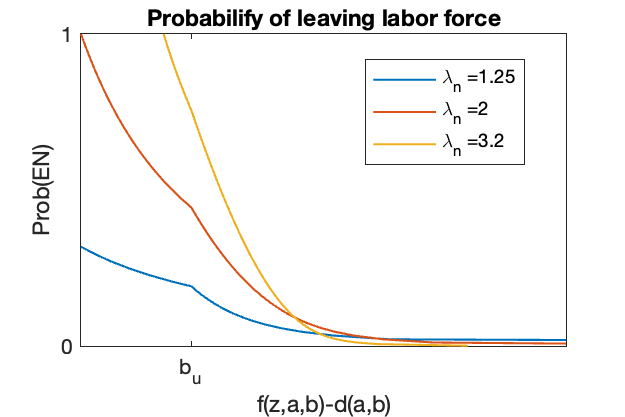
\includegraphics[width=0.48\textwidth]{Analytical2_2}
\caption{Different $\lambda$}
\label{Analytical1}
\end{figure}

\subsection{Value of vacancy}
In this section, I focus on the simple case where utility from leisure $b_u = 0$ so that I can have a simpler expression for vacancy value. Also, since $\lambda_n$ does not change the decision rule of accepting a job offer, I assume that $\lambda_n \to \infty$, the home productivity is constant $\epsilon_n = 0$. Unemployed workers are indifferent between staying in or leaving the labor force. In this case, the values of being unemployed and not in the labor force are zero: $V_u = V_n = 0$. If at the same time, the productivity shock is very persistent, $z' = z$ with probability very close to 1, $S(z,a,b)$, $P(z,a,b)$ and $D(z,a,b)$ can be approximately written as: 

\begin{align*}
S(z,a,b) &= 
\begin{dcases}
f(z,a,b)-d(a,b) &, f(z,a,b)-d(a,b)<0\\
\frac{f(z,a,b)-d(a,b)}{1-(1-\delta)\beta} &,  f(z,a,b)-d(a,b) \geq 0 \\
\end{dcases}\\
P(z,a,b) &= 
\begin{dcases}
f(z,a,b)&, f(z,a,b)-d(a,b)<0\\
\frac{f(z,a,b) }{1-(1-\delta)\beta} &,  f(z,a,b)-d(a,b) \geq 0\\
\end{dcases}\\
D(z,a,b) &= 
\begin{dcases}
d(a,b)&, f(z,a,b)-d(a,b)<0\\
\frac{d(a,b)}{1-(1-\delta)\beta} &,  f(z,a,b)-d(a,b) \geq 0 \\
\end{dcases}
\end{align*}

\begin{proposition}
If $a$ and $b$ are not too small, then there exists $\alpha_1^*(z), \alpha_2^*(z)$ such that the match is successful when $\frac{a}{b}\in(\alpha_1^*(z),\alpha_2^*(z))$. 
\end{proposition}
Given $z$ and $b$, $f(z,a,b)-d(a,b)$ is firstly increasing in $\frac{a}{b}$, then decreasing in $\frac{a}{b}$ when the mismatch penalty starts to dominate. The lower bound $\alpha_1^*$ is increasing in $\alpha_u$ and decreasing in $z$ and $\kappa$; while the upper bound $\alpha_2^*$ is decreasing in $\kappa$ and $\alpha_u$ and increasing in $z$. Higher productivity increases the probability of match success, while a higher mismatch penalty decreases the probability of match success. Higher return to labor $\kappa$ makes the match more tolerant towards over-qualification but more vulnerable towards under-qualification. 
\begin{figure}[h!]
\centering
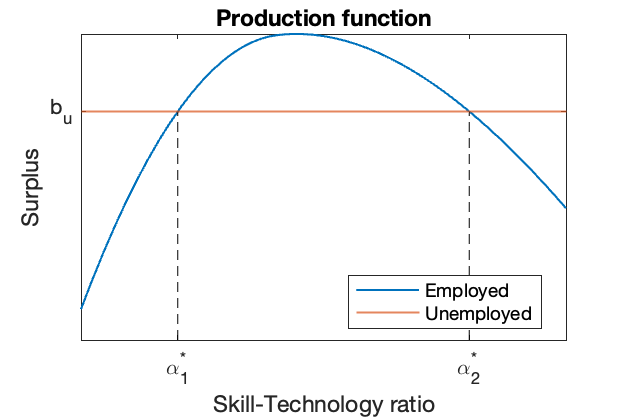
\includegraphics[width=0.48\textwidth]{Analytical1}
\caption{Different $\lambda$}
\label{Analytical1}
\end{figure}
\begin{align*}
\alpha_1^*(z) &= \frac{2\alpha_u+z\kappa-\sqrt{4z\alpha_u+(z\kappa)^2}}{2\alpha_u} \\
\alpha_2^*(z) &=\frac{2\alpha_o}{2\alpha_o+z(1-\kappa)-\sqrt{4z\alpha_o+(z(1-\kappa))^2}} 
\end{align*}

The measure of mismatch ($M$) is defines as the unconditional probability that the match is unsuccessful due to the over or under qualification. 
\begin{align*}
M(z,a,b) &= \int_a\int_b1\{f(z,a,b)-d(a,b) \leq 0\}d\Gamma_a(a)d\Gamma_b(b) \\
&= \frac{1}{\lambda_a+\lambda_b}\Big(\lambda_b(\frac{H}{\alpha_2^*(z)Q})^{\lambda_a}+\lambda_a(\frac{H}{\alpha_1^*(z)Q})^{-\lambda_b}\Big)
\end{align*}
\begin{proposition}
The mismatch level is minimized when 
\begin{align*}
\frac{H}{Q} = (\alpha_1^*(z)^{\lambda_b}\alpha_2^*(z)^{\lambda_a})^{\frac{1}{\lambda_a+\lambda_b}}
\end{align*}
\end{proposition}
The expected value of vacancy is related to the composition of unemployment. All the workers are facing the same job arriving rate, but with probability $\frac{M}{u}$, the match is unsuccessful; with probability $\frac{u-M}{u}$, the match is successful, and the expected value of vacancy $\Omega_u^*$  depends on the distribution of $a$ and $b$. 
\begin{align*}
\Omega_u &= \frac{u-M}{u}\Omega_u^* = \frac{(1-M)u^*}{M + (1-M)u^*}\Omega_u^* \\
\Omega_u^* &= \frac{(1-\delta)\beta}{1-(1-\delta)\beta}\frac{1}{1-M}\int_a\int_b\Big(f(z,a,b)-d(a,b)\Big)1\{f(z,a,b)-d(a,b)>0\}d\Gamma_a(a)d\Gamma_b(b) \\
				&=\frac{(1-\delta)\beta}{1-(1-\delta)\beta} \frac{1}{1-M}  (Eg(z,a,b)-Ep(z,a,b)-Ed(z,a,b))
\end{align*}

When $H$ and $Q$ are not too different, $\alpha_1^*(z)<\frac{H}{Q}<\alpha_2^*(z)$ for all $z$, the expected value of vacancy could be approximated as following: 
\begin{align*}
& Eg(z,a,b)= \int_a\int_bg(z,a,b)1\{f(z,a,b)-d(a,b)>0\}d\Gamma_a(a)d\Gamma_b(b) \\
&= z\Big(\kappa\frac{\lambda_a}{\lambda_a-1}H+(1-\kappa)\frac{\lambda_b}{\lambda_b-1}Q \\
&-\frac{\lambda_a\lambda_b}{\lambda_a+\lambda_b-1}\big(H^{\lambda_a}Q^{1-\lambda_a}(\frac{\kappa}{\lambda_a-1}+\frac{1-\kappa}{\lambda_a})\alpha_2^*(z)^{1-\lambda_a}+H^{1-\lambda_b}Q^{\lambda_b}(\frac{\kappa}{\lambda_b}+\frac{1-\kappa}{\lambda_b-1})\alpha_1^*(z)^{\lambda_b}\big)\Big)
\end{align*}
The expected output $Eg(z,a,b)$ can be decomposed into 2 parts. The first part is the aggregate production function. The second part is the unsuccessful match, which needs to be subtracted from the total output. While keeping average skill and technology level the same, the expected output $Eg(z,a,b)$ increases in $\lambda_a$ and $\lambda_b$, higher skill and technology variances increase the mismatch and reduces the expected output of the match.  \\

The expected penalty and disutility can be written as: 
\begin{align*}
Ep(z,a,b) &= \alpha_uQ \frac{\lambda_a\lambda_b}{\lambda_a+\lambda_b-1}(\frac{H}{Q})^{1-\lambda_b}\Big(\Lambda_b(1)-\Lambda_b(\alpha_1^*(z))\Big) \\
Ed(z,a,b) &= \alpha_oQ \frac{\lambda_a\lambda_b}{\lambda_a+\lambda_b-1}(\frac{H}{Q})^{\lambda_a}\Big(\Lambda_a(1)-\Lambda_a(\frac{1}{\alpha_2^*(z)})\Big) 
\end{align*}
While function $\Lambda_a(x)$ and $\Lambda_b(x)$ are defined as: 
\begin{align*}
\Lambda_a(x) &= \frac{x^{\lambda_a-1}}{\lambda_a-1}- \frac{2x^{\lambda_a}}{\lambda_a}+ \frac{x^{\lambda_a+1}}{\lambda_a+1}\\
\Lambda_b(x) &= \frac{x^{\lambda_b-1}}{\lambda_b-1}- \frac{2x^{\lambda_b}}{\lambda_b}+ \frac{x^{\lambda_b+1}}{\lambda_b+1}
\end{align*}
While keeping average skill and technology level the same, the expected penalty $Ep(z,a,b)$ and disutility $Ed(z,a,b)$ are decreasing in $\lambda_a$ and $\lambda_b$, higher skill and technology variance increase the mismatch penalty and disutility. When fixing technology level $Q$, the expected penalty $Ep(z,a,b)$ is decreasing in $\frac{H}{Q}$, and the expected disutiliy $Ed(z,a,b)$ is increasing in $\frac{H}{Q}$. 
\begin{proposition}
The deadweight loss caused by mismatch is minimized when 
\begin{align*}
\frac{H}{Q} = \Bigg(\frac{\alpha_u(\lambda_b-1)\Big(\Lambda_b(1)-\Lambda_b(\alpha_1^*(z))\Big)}{\alpha_o\lambda_a\Big(\Lambda_a(1)-\Lambda_a(\frac{1}{\alpha_2^*(z)})\Big)}\Bigg)^{\frac{1}{\lambda_a+\lambda_b-1}}
\end{align*}
\end{proposition}


\subsection{Level of unemployment}
The mismatch affects the unemployment rate through frictional unemployment (job finding rate) and mismatch unemployment (unsuccessful match due to mismatch penalty). The mismatch penalty lowers the expected surplus of creating an additional vacancy and the job-finding rate. It takes longer for the workers to get matched, and the frictional unemployment rate is higher. The mismatch penalty also turns the surplus of some matches negative, and workers reject the offer and stay unemployed. The mismatch unemployment depends on the probability of match surplus being negative. \\

The steady-state unemployment rate has two components, frictional unemployment ($u^*$) and mismatch unemployment ($M$). $u^*$ is a function of separation rate $\delta$ and job finding rate $\phi$. 
\begin{align}
\label{eqn:unemployment}
u = (1-M)u^*+M =  (1-M)\frac{\delta}{\delta+\phi}+M
\end{align}

The job finding rate $\phi$ can be solved using free entry condition of the firm, where $c$ is the cost of vacancy, $\theta$ is the job market tightness, and job arriving rate $\phi$ is a function of the market tightness. 
\begin{align*}
c\frac{\theta}{\phi(\theta)} = \frac{u-M}{u}\Omega_u^*
\end{align*}
The first component of unemployment is frictional unemployment. The mismatch penalty decreases the expected vacancy value $\Omega_u^*$ and.  The equilibrium job market tightness $\theta$ chosen by the firm is lower, and the job-finding rate $\phi(\theta)$ is lower. The equilibrium frictional unemployment rate $u^* =\frac{\delta}{\delta+\phi}$ is then higher. \\

The second component is mismatch unemployment. Mismatch penalty turns the surplus of some matches to be negative, with probability $M$, workers get mismatched and will stay unemployed even if job arrives.  \\

In a standard DMP model, the job arriving rate responds to the labor productivity shock through free entry conditions. The job-finding rate responds less to TFP shocks with mismatch penalties. When Total Factor Productivity (TFP) is higher, more matches will receive mismatch penalty (extensive margin), and the average mismatch penalty received is higher (intensive margin).  The expected surplus of creating an additional vacancy $\Omega_u^*$ is calculated based only on the successful matches. As plotted in figure \ref{Analytical3} (left), the change rate of vacancy value with respect to TFP is lower when matches receive mismatch penalty than when there is no mismatch penalty. At the same time, when TFP is high, firms create more jobs. A higher job arriving rate decreases the frictional unemployment rate $u^*$, then high-skilled workers are more likely to get matched and become employed. The firms are more likely to get matched with low-skilled workers, and the matches are more likely to fail. The lower net expected value of vacancy $\Omega_u = \frac{(1-M)u^*}{M + (1-M)u^*}\Omega_u^*$ decreases firm's job creation. \\

The mismatch penalty increases unemployment volatility mainly through the mismatch unemployment fluctuation. As plotted in figure \ref{Analytical3} (right), the measure of mismatch (probability of unsuccessful match) is decreasing in TFP. It linearly affects the unemployment rate $u = M + (1-M)u^*$. The response is asymmetric; the mismatch unemployment will respond more to a negative TFP shock.  \\

\begin{figure}[h!]
\centering
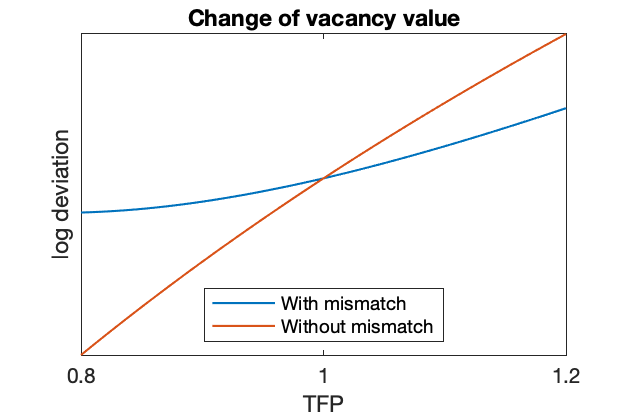
\includegraphics[width=0.48\textwidth]{Analytical3}
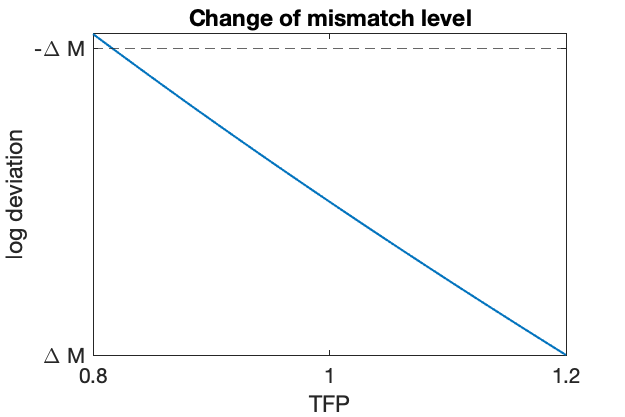
\includegraphics[width=0.48\textwidth]{Analytical4}
\caption{Deviation with respect to TFP shocks}
\label{Analytical3}
\end{figure}

\subsection{Efficiency}
In the decentralized market, the job-finding rate $\phi$ can be solved using the free entry condition of the firm, where $c$ is the cost of vacancy, $\theta$ is the job market tightness. Job arriving rate $\phi$ is a function of the market tightness. 
\begin{align*}
c\frac{\theta}{\phi(\theta)} = \frac{u-M}{u}\Omega_u^* 
\end{align*}
Suppose that the social planner can create vacancies at the same cost $c$ as the decentralized market, subject to the same matching function. Given the current unemployment rate, he chooses a market tightness $\theta$ to maximize the social surplus, i.e., the total market output of employed workers, minus the total costs of vacancy creation, plus the continuation value. 
\begin{align*}
V(u) = \max_{\theta,u'}\quad (1-u)(1-\delta)\E(f(z,a,b)-d(a,b))-c\theta u+\beta V(u')
\end{align*}
subject to 
\begin{align*}
u' = u+(1-u)\delta-(u-M)\phi(\theta)
\end{align*}
By solving first order condition, at steady state, the optimal vacancy creation needs to satisfy:
\begin{align*}
c\frac{\theta}{\phi(\theta)} &= \frac{u-M}{u}\alpha\lambda 
\end{align*}
While $\lambda$ is the marginal social benefit of an additional employed worker: 
\begin{align*}
\lambda =\Omega_u^*-\underbrace{\beta\frac{\frac{M}{u}\phi(\theta)}{1-(1-\delta)\beta+\beta\phi(\theta)}\Omega_u^*}_{\text{mismatch externality}} -\underbrace{\beta\frac{\frac{u-M}{u}\phi(\theta)\Omega_u^*-c\theta}{1-(1-\delta)\beta+\beta\phi(\theta)}}_{\text{future value}}
\end{align*}

In the decentralized market, agents do not internalize the value of future matches and solve a static problem. The social planner solves a dynamic problem by taking into consideration future social welfare. In addition to the standard externality related to the frictional matching, a new externality, mismatch externality, arises. With mismatch, the low unemployment rate increases the probability of matching failure and decreases the vacancy creation incentive for the social planner. 

\begin{proposition}
Too many vacancies are created in the decentralized market, which decreases the job-finding rate, especially when the mismatch level is high.
\end{proposition}
The overall social value is lower than the firm's private value, and the difference is increasing in the mismatch level $M$. In the decentralized market, the firms create vacancies above the optimal level. 
\begin{align*}
\frac{\alpha\lambda}{\Omega_u^*} = \alpha\frac{(1-(1-\delta)\beta)\Omega_u^*+\beta c \theta}{(1-(1-\delta)\beta)\Omega_u^*+\beta c \theta\frac{u}{u-M}}<1
\end{align*}
When there are too many vacancies created, the job-finding rate $\phi(\theta)$ is higher. However, the effective job-finding rate $\frac{u-M}{u}\phi(\theta)$ is lower because of unsuccessful matches. The effective job-finding rate $\frac{u-M}{u}\phi(\theta)$ can be written as a function of job-finding rate $\phi(\theta)$ using equation (\ref{eqn:unemployment}). The effective job-finding rate is decreasing in job-finding rate and mismatch level. 
\begin{align*}
\frac{u-M}{u}\phi(\theta) = \frac{1}{1+\frac{M}{1-M}\frac{\delta+\phi(\theta)}{\delta}}
\end{align*}

\begin{proposition}
The decentralized economy has too high an unemployment exit rate. 
\end{proposition}
Due to the wage determination mechanism, the agents fail to internalize the value of the future matches. The social values of unemployment and employment (demoted with stars) are different from the private values because they internalize the value of future matches. The value of unemployment depends on the skill level and the current productivity level, because they affect the quality of future matches for the worker. It also depends on the job-finding rate because it affects how likely the worker can get matched in the future. The match surplus is lower in the social planner's problem; the social planner will reject some matches accepted by the decentralized market. 

\begin{align*}
V_u^*(z,a) &= \frac{\beta\Phi\theta^{\alpha}}{1-\beta}\E \max\{S^*(z,a,b),0\} \\
S^*(z,a,b) &= 
\begin{dcases}
S(z,a,b)-(1-\beta) V_u^*(z,a)&, S^*(z,a,b)<0\\
S(z,a,b)-\frac{(1-\beta) V_u^*(z,a)}{1-(1-\delta)\beta} &,  S^*(z,a,b) \geq 0 \\
\end{dcases}
\end{align*}

\section{Extended Model: Endogenous skill and technology}
In the extended model, I still consider the case where the skill and technology does not depreciate: $\delta_a = \delta_b = 0$. There is no on-the-job search $s=0$. However, I allow the skill and technology to be endogenous by assuming that the cost of training and technology adoption are finite: $\phi_a<\infty$ and $\phi_b<\infty$. To be able to have a closed-form solution, I still need to assume that $\lambda_n \to \infty$ and the productivity shock is very persistent: $z' = z$ with probability very close to 1. \\

Once the match is formed successfully, the worker and the firm can adjust their skill and technology level for the new match. The adjustment is a convex function of the adjustment level, $\phi_a(a'-a)^2/a$ for skill and $\phi_b(b'-b)^2/b$ for technology. The cost of training could be interpreted as time spent on training instead of working or the cost associated with a classroom-style training. The cost of technology adoption could be interpreted as the money spent on new patents or new equipments. 

\subsection{Optimal skill and technology level}
The value of new match is the maximized total surplus minus the cost of technology adoption and training: 
\begin{align*}
\bar{S}(z,a,b) = \max _{a^*,b^*} \quad (1-\delta)\beta S(z,a^*,b^*)-\phi_a\frac{(a^*-a)^2}{a}-\phi_b\frac{(b^*-b)^2}{b}
\end{align*}
The optimal skill and technology level could be solved as: 
\begin{align*}
\alpha_{i-1}(z) \leq \frac{a}{b}<\alpha_{i}(z), \quad a^*= r_{ai}(z,\frac{a}{b})a, \quad b^*= r_{bi}(z,\frac{a}{b})b, 
\end{align*}
Define $\tilde{\phi}_a = \frac{1-(1-\delta)\beta}{(1-\delta)\beta}\phi_a$, $\tilde{\phi}_b =\frac{1-(1-\delta)\beta}{(1-\delta)\beta}\phi_b$ and $\Phi(z) = \tilde{\phi}_a+\tilde{\phi}_b+\frac{1}{2}z$, then $\alpha_{i}$ could be solved as: 
\begin{align*}
&\alpha_0(z)= 0,
&&\alpha_1(z) = \frac{\alpha_u\tilde{\phi}_a-\frac{1}{2}z(1-\kappa)\tilde{\phi}_a}{\alpha_u(\tilde{\phi}_a+\frac{1}{2}z)},  \\
&\alpha_2(z) = \frac{\tilde{\phi}_a\tilde{\phi}_b+\frac{1}{2}z(1-\kappa)\tilde{\phi}_a}{\tilde{\phi}_a\tilde{\phi}_b+\frac{1}{2}z\kappa\tilde{\phi}_b},
&&\alpha_3(z) = \frac{\alpha_o(\tilde{\phi}_b+\frac{1}{2}z)}{\alpha_o\tilde{\phi}_b-\frac{1}{2}z\kappa\tilde{\phi}_b}, 
&&\alpha_4(z) = \infty 
\end{align*}
$r_{ai}$ and $r_{bi}$ could be solved as: 
\begin{align*}
&r_{a1}(z,\frac{a}{b}) = \frac{\tilde{\phi}_a+\frac{1}{2}z\kappa+\alpha_u}{\tilde{\phi}_a+\alpha_u\frac{a}{b}}, 
&&r_{b1}(z,\frac{a}{b})= 1\\
&r_{a2}(z,\frac{a}{b}) = \frac{\tilde{\phi}_a\tilde{\phi}_b+\frac{1}{2}\tilde{\phi}_bz\kappa+\Phi\alpha_u}{\tilde{\phi}_a\tilde{\phi}_b+(\tilde{\phi}_a+\tilde{\phi}_b\frac{a}{b})\alpha_u}, 
&&r_{b2}(z,\frac{a}{b})=  \frac{\tilde{\phi}_a\tilde{\phi}_b+\frac{1}{2}\tilde{\phi}_az(1-\kappa)+\Phi\alpha_u\frac{a}{b}}{\tilde{\phi}_a\tilde{\phi}_b+(\tilde{\phi}_a+\tilde{\phi}_b\frac{a}{b})\alpha_u}\\
&r_{a3}(z,\frac{a}{b}) = \frac{\tilde{\phi}_a\tilde{\phi}_b+\frac{1}{2}\tilde{\phi}_bz\kappa+\Phi\alpha_o\frac{b}{a}}{\tilde{\phi}_a\tilde{\phi}_b+(\tilde{\phi}_a\frac{b}{a}+\tilde{\phi}_b)\alpha_o}, 
&&r_{b3}(z,\frac{a}{b})=  \frac{\tilde{\phi}_a\tilde{\phi}_b+\frac{1}{2}\tilde{\phi}_az(1-\kappa)+\Phi\alpha_o}{\tilde{\phi}_a\tilde{\phi}_b+(\tilde{\phi}_a\frac{b}{a}+\tilde{\phi}_b)\alpha_o}\\
&r_{a4}(z,\frac{a}{b}) = 1, 
&&r_{b4}(z,\frac{a}{b})= \frac{\tilde{\phi}_b+\frac{1}{2}z(1-\kappa)+\alpha_o}{\tilde{\phi}_b+\alpha_o\frac{b}{a}}
\end{align*}

The upgrade decision depends on the current TFP $z$, and skill-technology mismatch level $\frac{a}{b}$. Workers and firms tend to decrease the measure of mismatch $|\frac{a}{b}-1|$ in order to avoid the penalty while upgrading their skill and technology level to improve productivity. When the cost of training $\phi_a$ and technology adoption $\phi_b$ are similar, the adjustment of skill and technology is more balanced, the measure of mismatch $|\frac{a}{b}-1|$ after adjustment is small. If there is a great difference between the cost of technology adoption and training, for example, $\phi_b<<\phi_a$, technology will be adjusted more than training, and $|\frac{a}{b}-1|$ will be large, especially when TFP $z$ is high, the productivity gain from adjustment is large.    

\begin{proposition}
The technology and training decision is pro-cyclical; when the aggregate productivity $z$ is high, skill and technology are more likely to be upgraded (extensive margin), and the upgraded level will be higher (intensive margin). 
\end{proposition}
Skill and technology will be upgraded the same time when $\frac{a}{b} \in (\alpha_1,\alpha_3)$, while $\alpha_1$ is decreasing in $z$ and $\alpha_3$ is increasing in $z$. Given $\frac{a}{b}$, $r_{a}$ and $r_{b}$ are both increasing in $z$. 

\begin{proposition}
The endogenous technology adoption and training decision increases mismatch during the recession if there exists $z_2>z_1$ and $\alpha_0$ such that 
\begin{align*}
\frac{r_a(\alpha_0,z_1)}{r_b(\alpha_0,z_1)}\alpha_0>\alpha_1(z_1), \quad \frac{r_a(\alpha_0,z_2)}{r_b(\alpha_0,z_2)}\alpha_0<\alpha_1(z_1)
\end{align*}
or 
\begin{align*}
\frac{r_a(\alpha_0,z_1)}{r_b(\alpha_0,z_1)}\alpha_0<\alpha_2(z_1),\quad \frac{r_a(\alpha_0,z_2)}{r_b(\alpha_0,z_2)}\alpha_0>\alpha_2(z_1)
\end{align*}
\end{proposition}
As plotted in figure \ref{Analytical5}, the match is successful between dash line $\alpha_1^*$ and $\alpha_2^*$ given low TFP. Suppose the initial match ratio is $\frac{a}{b} = \alpha_0$. If the skill and technology adjustment decision is made when TFP is low (blue line), the match will be successful after the adjustment is made. However, if the adjustment decision is instead made when TFP is high (red line), the firm will choose a much higher technology level to maximize the output, the match is optimal when TFP is high, but it won't be successful when the TFP is low.  

\begin{figure}[h!]
\centering
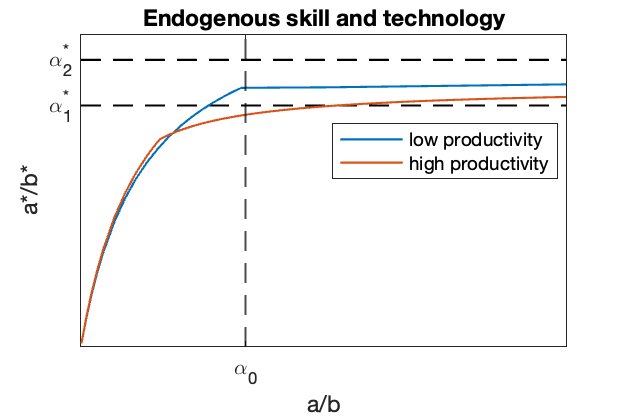
\includegraphics[width=0.48\textwidth]{Analytical5}
\caption{Endogenous skill and technology}
\label{Analytical5}
\end{figure}

\subsection{Efficiency}
As discussed in the previous chapter, the value function of social planner is different from that of decentralized market because the planner will internalize the value or future matches. 
\begin{align*}
V_u^*(z,a) &= \frac{\beta\Phi\theta^{\alpha}}{1-\beta}\E \max\{S^*(z,a,b),0\} \\
V_e^*(z,a,b) &= 
\begin{dcases}
f(z,a,b)-d(a,b)+\beta V_u^*(z,a)&, V_e^*(z,a,b)<V_u^*(z,a)\\
\frac{f(z,a,b)-d(a,b)+\delta\beta V_u^*(z,a)}{1-(1-\delta)\beta} &,  V_e^*(z,a,b) \geq V_u^*(z,a) \\
\end{dcases}
\end{align*}

\begin{proposition}
Given current TFP and technology distribution, there exists a threshold $a_u^{*}(z)$ such that unemployed workers with skill level below $a_u^{*}(z)$ underinvest in training. Given current TFP, technology distribution and matched firm's technology level, there exist a threshold $a_e^{*}(z,b)$ such that employed workers with skill level below $a_e^{*}(z,b)$ underinvest in training.
\end{proposition}

The unemployed workers do not invest in their training in the decentralized market. However, the social planner solves the following maximization problem, and provides positive training if and only if $d V_u^*(z,a)/d a>0$
\begin{align*}
\bar{V}_u^*(z,a) = \max_{a^*} \quad V_u^*(z,a)-\phi_a\frac{(a^*-a)^2}{a}
\end{align*}

Given current TFP and technology distribution, $V_u^*(z,a)$ firstly increases in $a$ when the productivity gain dominates, then decreases in $a$ when the disutility dominates. There exists a threshold $a_u^{*}(z)$ such that $d V_u^*(z,a)/d a>0$ when $a<a_u^{*}(z)$. The social planner provides positive training to workers with skill level below $a_u^{*}(z)$. \\

For the employed workers, the social planner solves the following problem to maximize the social surplus of a match. The investment in training changes not only the expected value of the current surplus, but also the value of the worker when he gets separated from the firm. 
\begin{align*}
\bar{V}_e^*(z,a,b) &= \max_{a^*,b^*} \quad (1-\delta)\beta V_e^*(z,a^*,b^*)+\delta\beta V_u^*(z,a)-\phi_a\frac{(a^*-a)^2}{a}-\phi_b\frac{(b^*-b)^2}{b} \\
 &= \max_{a^*,b^*} \quad (1-\delta)\beta S(z,a^*,b^*)+\frac{\delta\beta V_u^*(z,a^*)}{1-(1-\delta)\beta}-\phi_a\frac{(a^*-a)^2}{a}-\phi_b\frac{(b^*-b)^2}{b}
\end{align*}
At the optimal skill and technology level chosen in the decentralized market, $d\bar{S}^*(z,a,b)/d a^* \leq 0 $:  
\begin{align*}
\frac{d\bar{S}^*(z,a,b)}{d a^*} = \kappa-2\phi_a\frac{a^*-a}{a} &-2\alpha_u\frac{a^*-b^*}{b}1\{a^*<b^*\}	\\
																									&-2\alpha_o\frac{a^*-b^*}{a}1\{a^*>b^*\}
\end{align*}
Take derivative on $\bar{V}_e^*(z,a,b)$ with respect to $a^*$: 
\begin{align*}
\frac{d\bar{V}_e^*(z,a,b)}{d a^*}  & = \frac{d\bar{S}^*(z,a,b)}{d a^*} + \frac{\delta\beta}{1-(1-\delta)\beta}\frac{d V_u^*(z,a^*)}{d a^*} 
\end{align*}
The social planner will provide more training if and only if $d\bar{V}_e^*(z,a,b)/d a^*>0$. There exists a threshold $a_e^{*}(z,b)$ such that $d\bar{V}_e^*(z,a,b)/d a^*>0$ when $a<a_e^{*}(z,b)$. The social planner provides positive training to workers with skill level below $a<a_e^{*}(z,b)$, and $a_e^{*}(z,b)$ is increasing in $b$.  \\



\section{Calibration}
In this section, I solve the full model numerically and estimate the model using the Simulated Method of Moments (SMM). The human capital and technology depreciation rates are positive, $\delta_a>0$ and $\delta_b>0$; the on-the-job search efficiency is greater than zero, $s>0$; and the aggregate productivity persistency is less than 1, $\rho_z<1$. \\

The total surplus $S(z,a,b)$, the expected net output $P(z,a,b)$ and the expected disutility $D(z,a,b)$ of the match could be solved as: 
\begin{align*}
S(z,a,b) &= f(z,a,b)-d(a,b)-b_u \\
			 &+(1-\delta)\beta \E_{z',b'|z,b}\max\{\E_{\epsilon_n}\max\{S(z',a,b')+b_u,\epsilon_n\}-\E_{\epsilon_n}\max\{b_u,\epsilon_n\},0 \}  \\
D(z,a,b) &=V_u+d(a,b)+(1-\delta)\beta \E_{z',b'|z,b}\E_{\epsilon_n}(D(z',a,b')-V_u)1\{{S(z',a,b')+b_u>\max\{b_u,\epsilon_n\}}\} \\
P(z,a,b) &= S(z,a,b)+D(z,a,b) \\
\end{align*}
Where $\log z$ follows an AR(1) process $\log z' = \rho_z \log z +\epsilon_z$
The expected value of new match is the maximized total surplus minus the cost of technology adoption and training: 
\begin{align*}
\E\bar{S}(z,a,b) = (1-\delta)\beta\max _{a^*,b^*}  \E_{z'|z,a',b'}S(z,a^*,b^*)-\phi_a\frac{(a^*-a)^2}{a}-\phi_b\frac{(b^*-b)^2}{b}
\end{align*}
Then we can solve the expected profit the firm can get by hiring the worker. 
\begin{align*}
\Omega_u(z) &= (1-\delta)\beta\int_a \int_b \max\{\E\bar{S}(z,a,b),0\}u(a)\gamma_b(b)dbda \\
\Omega_e(z,L) &= (1-\delta)\beta\int_a\int_b\int_{b'}\max\{\E S(z,a,b)-\E S(z,a,b'),0\}l(a,b')\gamma_b(b)db'dbda 
\end{align*}
The free entry condition can be written as: 
\begin{align*}
\kappa \frac{\theta(z,L)}{\phi(\theta(z,L))} =  \frac{u \Omega_u(z)+s(1-u)\Omega_e(z,L)}{u+s(1-u)} 
\end{align*}

\subsection{Calibration form literature}
For the standard parameters related to labor market and depreciation, I used the calibration form literature. Values I use are listed in table \ref{Calibration1}. \\

\begin{table}[h!]
\begin{tabular}{llll}
\hline \hline
Parameter     &       Description      & Calibration &  Value                    \\
\hline 
$\beta$ & Discount rate & MPV(2018) & 0.995 \\
$\rho_z$   &  AR(1) process for log TFP & MPV(2018) & 0.947 \\
$\sigma_z$ &  AR(1) process for log TFP & MPV(2018) & 0.0067 \\
$s$ & OJS efficiency & MPV(2018) & 0.176\\
$\alpha$ & Matching function elasticity & MPV(2018) & 0.5\\
$b_u$ & Utility from leisure & MPV(2018) & 0.75\\
$\delta$ & Exogenous separation rate & MPV(2018) & 0.024 \\
$\delta_a$ & Human capital depreciation rate & Arrazola and Hevia (2004) & 0.015\\
$\delta_b$ & Technology depreciation rate & Li and Hall(2016) & 0.02\\
$c$ & Cost of vacancy & Unemployment rate \\
\hline 
\end{tabular}
\caption{Calibration form literature}
\label{Calibration1}
\end{table}

For parameters for TFP $\rho_z$ and $\sigma_z$, discount rate ($\beta$), elasticity of matching function ($\alpha$), search efficiency of employed worker ($s$) and utility from leisure ($b$), I use the calibration from MPV(2018)\cite{MPV2018}. I set $\rho_z = 0.947$, $\sigma_z = 0.0067$, $\beta = 0.95^{\frac{1}{12}}$, $\alpha = 0.5$, $s = 0.176$ and $b = 0.75$. \\

Li and Hall(2016)\cite{LiHall2016} estimated the annual depreciation rate of R\&D capital, which is around 20\%-40\% for most of the sectors, so I use 2\% as technology monthly depreciation rate. Arrazola and Hevia (2004)\cite{ArrazolaHevia2004} use the European Household Panel to estimate the rate of depreciation of human capital, the results show depreciation rates are between 1\% and 1.5\%. G{\"o}rlich and De Grip (2008)\cite{GorlichDeGrip2008} use German Socio-Economic Panel to estimate human capital depreciation rates during career interruptions. Based on Mincer’s earnings function, the estimation results show that long-run unemployment decreases the wage by 1.5\%, while short-run decreases by 0.2\%. I use 1.5\% as the human capital monthly depreciation rate. \\


\subsection{Simulated Method of Moments}
The remaining parameters to calibrate are home productivity shock distribution $\lambda_n$, capital return $\kappa$, under and over qualification penalty $\alpha_u$ and $\alpha_o$, skill and technology volatility $\lambda_a$ and $\lambda_b$, skill and technology shock probability $P_a$ and $P_b$, and cost of technology adoption and training $\phi_a$ and $\phi_b$. To estimate, I use the Simulated Method of Moments (SMM), which aims at finding a value $\theta^*$ maximizing the likelihood function. 
\begin{align*}
L(\theta) = -(\hat{m}_S-\hat{m}_M)^T(\hat{m}_S-\hat{m}_M)
\end{align*}
where $\hat{m}_S$ is the moment simulated by model given $\theta$ as the parameter of the model; $\hat{m}_M$ is the moment observed in the data. 

The home productivity shock distribution ($\epsilon_{min}$ and $\lambda_n$) is calibrated to match the labor flow in the data: Labor force participation rate (LFPR), employment, unemployment, and not-in-Labor-Force to not-in-Labor-Force (EN, UN, NN) transition in the data. Given $\lambda_n$, $\epsilon_{min}$ can be pinned down by matching the unemployment and not-in-Labor-Force to not-in-Labor-Force transition $UN+NN = (\epsilon_{min}/b_u)^{\lambda_n}$. $\lambda_n$ determines the dispersion of the home production and is calibrated to match the employment to not-in-Labor-Force transition (EN). \\

The average hours spent on formal training per week is 0.6 hours, which is around 2\% of the working hours. I use 2\% as the ratio between the training cost and the revenues. Training is also related to wage growth. Barron et al.(1989)\cite{Barronetal1989
} use EOPP to study the on-the-job training. They found that a 10\% increase in training is associated with a 3\% increase in productivity growth and a 1\% increase in wage growth. Frazis and Loewenstein (2006)\cite{FrazisLoewenstein2006} used EOPP data to estimate the wage growth corresponding to the productivity change, the productivity growth of 10 percent results in wage growth of only 2.6 percent. So I also match the model with the wage dynamics summarized in Lise et al.(2013)\cite{Liseetal2013} using NLSY monthly data.  \\

Technology diffusion survey data by Bartel et al.(2009)\cite{Barteletal2009}, Business R\&D and Innovation Survey (BRDIS), Business Enterprise Research and Development (BERD), and Compustat can be used to estimate the cost of technology adoption. According to BRDIS(2006), the Worldwide R\&D paid for by the company is around 4\% of Worldwide net sales and operating revenues. I use 4\% as the ratio between the technology adoption cost and the revenues.\\

To calibrate the parameters for the production function and skill and technology distribution. I match the moment of the wage distribution estimated by Song et al.(2018)\cite{Songetal2018}: the between firm variance, the within-firm variance, and the covariance between firm's fixed effect and worker's fixed effect. The variance of worker's fixed effect and the covariance between worker and firm can be decomposed as: 
\begin{align*}
& \var(a) =\var(WFE) + \var(XB) +\var(\epsilon) \\
& \cov(a,b) = \cov(WFE,FFE)+\cov(Xb,FFE)
\end{align*}

All the moments I try to match are summarized in table \ref{Summary_moment}. \\

\begin{table}[h!]
\centering
\begin{tabular}{l|lll}

\hline \hline
Moments            & 1980-1986     & 2007-2013      		\\
\hline 
Unemployment		&	0.055	&	0.055 		\\
LFPR 						& 0.65 		&0.65 			\\
EU							& 0.035	&0.035 		\\
EE 							& 0.02 		& 0.02			\\
EN     						& 0.017 	& 0.017     	\\
UN+NN 					& 0.31 		& 0.35        	\\
\hline
\multicolumn{4}{c}{\small Data source: FRED} \\
\multicolumn{4}{c}{} \\
\hline
Moments            & 1980-1986     & 2007-2013      		\\
\hline 
Labor share     & 0.64 & 0.58        						\\
\hline
\multicolumn{4}{c}{\small Data source: BLS} \\
\multicolumn{4}{c}{} \\
\hline 
Moments   &      Value       \\
\hline 
Training/Working hour  & 2\%   \\
R\&D/Revenue & 4\%  \\
\hline 
\multicolumn{4}{c}{\small Data source: EOPP and BRDIS} \\
\multicolumn{4}{c}{} \\
\hline 
Wage Moment           & 1980-1986     & 2007-2013      		\\
\hline 
$\var(\omega)$    & 0.708         & 0.924                             \\
$\var(a)$              & 0.538(76.1\%) & 0.671(72.6\%)   	\\
$\var(b)$             & 0.084(12\%)   & 0.081(9\%)             \\
$2\cov(a,b)$          & 0.055(8\%)    & 0.135(15\%)           	\\
$\corr(a,b)$        & 0.13  	& 0.29           						\\
\hline
\multicolumn{4}{c}{\small Data source: Song et al.(2018)\cite{Songetal2018}} \\
\multicolumn{4}{c}{} \\
\hline 
Wage dynamics         & Less than HS & High School & College \\
\hline 
Employment rate                & 0.75                  & 0.85        & 0.94    \\
Change jobs given employment   & 0.04                  & 0.024       & 0.013   \\
Within Job Wage Growth        & 0.0026                & 0.0025      & 0.0021  \\
Var of within job wage growth & 0.0049                & 0.0038      & 0.003   \\
Between Job Wage Growth      & 0.082                 & 0.08        & 0.1     \\
Var of between job wage growth & 0.064                 & 0.062       & 0.058   \\
\hline 
\multicolumn{4}{c}{\small Data source: Lise et al.(2013)\cite{Liseetal2013}} \\
\end{tabular}
\caption{Summary of the moments}
\label{Summary_moment}
\end{table}

\subsection{Calibration Result}
The estimated value for the parameters are listed in table \ref{Parameter}. The labor market condition in 2007-2013 is different from that in 1980-1986 mainly in three ways: (1) the labor return in production function is lower in 2007-2013; (2) the skill dispersion was higher in 2007-2013; (3) the technology adoption cost was lower in 2007-2013. 

\begin{table}[h!]
\centering
\begin{tabular}{ll|cc}
\hline \hline
Parameter     &       Description         & 1980-1986     & 2007-2013                \\
\hline 
$\epsilon_{min}$& Home productivity level & 3.5067  & 3.5067 \\
$\lambda_n$& Home productivity dispersion & 3.5067  & 3.5067 \\
$\kappa$ & Return to skill & 0.6327  & 0.469    \\
$\alpha_u$ & Under-qualification penalty & 21.094  & 24.5333 \\
$\alpha_o$ & Over-qualification penalty & 29.8208 & 32.2478 \\
$\lambda_a$ & Skill dispersion & 6.952   & 4.0519   \\
$\lambda_b$ & Technology dispersion & 8       & 8       \\
$P_a$ & Skill shock probability & 0.6754  & 0.6754   \\
$P_b$ & Technology shock probability & 0.2727  & 0.2727   \\
$\psi_a$ & Cost of training & 8.9064  & 8.9064   \\
$\phi_b$ & Cost of technology adoption & 0.9206  & 0.5687  \\
\hline 
\end{tabular}
\caption{Parameter values}
\label{Parameter}
\end{table}

The calibration results for 1980-1986 and 2007-2013 respectively are presented in table \ref{Calibration_Result}. 
\begin{table}[h!]
\centering
\begin{tabular}{l|llll}
\hline \hline
           & \multicolumn{2}{c}{1980-1986}     & \multicolumn{2}{c}{2007-2013}                \\ 
            & Data     &  Model   & Data     &  Model     \\ \hline
Targeted moments  \\
Unemployment rate          & 0.055 & 0.1142 & 0.055 & 0.1580 \\
Labor force participation rate            & 0.65  & 0.6541 & 0.65  & 0.5462 \\
Job-to-Job transition       & 0.02  & 0.002 & 0.02  & 0.029 \\
Separation rate          & 0.35  & 0.0259 & 0.35  & 0.0258 \\
Return to labor        & 0.64  & 0.6693 & 0.58  & 0.5366 \\
Within-job wage growth      & 0.003 & 0.0033 & 0.003 & 0.0028 \\
Between-job wage growth    & 0.08  & 0      & 0.08  & 0.0007      \\
Skill and technology variance ratio          & 6.4   & 2.0311 & 8.28  & 2.9958 \\
Skill and technology correlation        & 0.13  & 0.1425 & 0.29  & 0.2963  \\
Training expense and revenues ratio & 0.03  & 0.011   & 0.03  & 0.007  \\
R\&D expense and revenues ratio  & 0.025 & 0.013  & 0.04  & 0.038 \\
\hline
Non targeted moments                  \\
Unemployment rate volatility          & 0.21  & 0.0533  & 0.28  & 0.0523 \\
Separation rate volatility           & 0.15  & 0.1175 & 0.15  & 0.1243 \\
Mismatch && 0.1232 &&0.4060 \\
\hline 
\end{tabular}
\caption{Calibration Result}
\label{Calibration_Result}
\end{table}

\begin{table}[h!]
\centering
\begin{tabular}{ll|ccc}
\hline \hline
Parameter     &       Description         & 1980-1986     & 2007-2013   & Mismatch             \\
\hline 
$\kappa$ & Return to skill & 0.6327  & 0.469 & 0.1193 \\
$\lambda_a$ & Skill dispersion & 6.952   & 4.0519 &  0.1422 \\ 
$\alpha_u$ & Under-qualification penalty & 21.094  & 24.5333 & \multirow{2}{*}{0.3540}\\
$\alpha_o$ & Over-qualification penalty & 29.8208 & 32.2478 \\
$\phi_{b}$ & Cost of technology adoption & 0.9206  & 0.5687 & 0.1326 \\
\hline 
\end{tabular}
\caption{Mismatch breakdown}
\label{Breakdown}
\end{table}

\subsection{Policy Analysis}
The mismatch creates deadweight loss and causes market failure. Firstly, matches are random, firms are not matched to the most suitable workers, and matches receive mismatch penalties on the output. Secondly, too many vacancies are created, not only because the agents fail to internalize the value of the future matches (the wage is determined by Bertrand competition), but also because the low unemployment increases the probability of matching failure. Thirdly, the agents underinvest in worker's training, both employed or unemployed. As a result, the mismatch level is higher, especially when technology adoption cost is low. Also, when a worker gets separated from his job, his human capital starts to depreciate; if the worker stays unemployed or out-of-labor-force for an extended period of time, the depreciated human capital makes it hard for him to find a job again.  \\

There are several possible ways to increase market efficiency. The first way is to increase unemployment insurance. By increasing unemployment insurance, the matching quality can be improved. Workers will be more patient when job opportunities arrive and wait until they get a match good enough. More workers will actively search for the job instead of leaving the labor force and have a chance to get matched. Also, fewer vacancies will be created since the firms will need to offer a higher salary to get the workers to accept the job, and the expected value of vacancy will be lower. The policy simulation result is plotted in figure \ref{Simulation1}. Even though the unemployment rate is higher with higher unemployment insurance (higher offer rejection rate), the overall employment level and quality are higher (higher labor force participation rate), and the total output is higher.

\begin{figure}[h!]
\centering
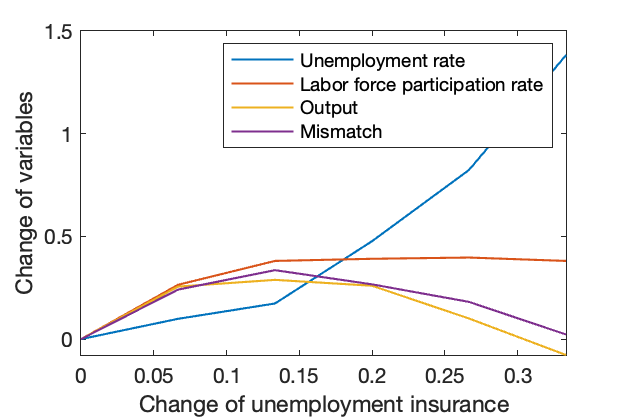
\includegraphics[width=0.48\textwidth]{Simulation1}
\caption{Policy experiment: Unemployment Insurance}
\label{Simulation1}
\end{figure}

Another way to improve the efficiency is to subsidize the training. With a lower cost of training, agents invest more in training; the difference between the skill and technology will then be smaller. Also, when a worker becomes unemployed with a higher skill level, he has a higher chance of finding a job before his skill depreciates too much. The policy simulation result is plotted in figure \ref{Simulation2}. Subsidies to the training increase the labor force participation rate and decrease the unemployment rate. Subsidies to the training also lower the mismatch level and increase the output level. 
\begin{figure}[h!]
\centering
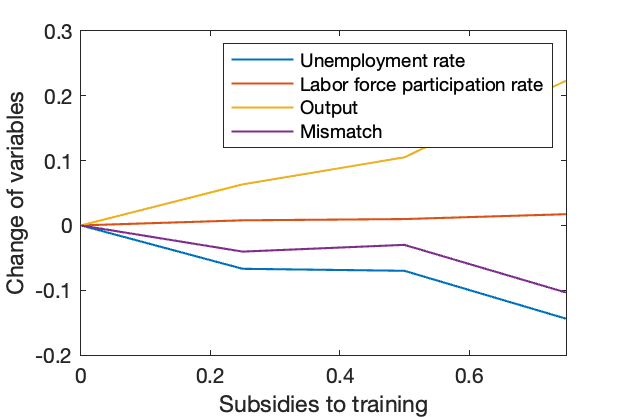
\includegraphics[width=0.48\textwidth]{Simulation2}
\caption{Policy experiment: Training subsidies}
\label{Simulation2}
\end{figure}

\section{Empirical Evidence}
\subsection{Slow overall recovery}
Compared with previous recessions, the slow employment recovery in the Great Recession is notable. As shown in figure \ref{Employment}, it took 31, 46, and 77 months to recover to the pre-recession employment level for the 1990 recession (July 1990-Mar 1991), the 2001 recession (March 2001-November 2001), and the 2008 recession (December 2007-June 2009), respectively. \\


\begin{figure}[h!]
\centering
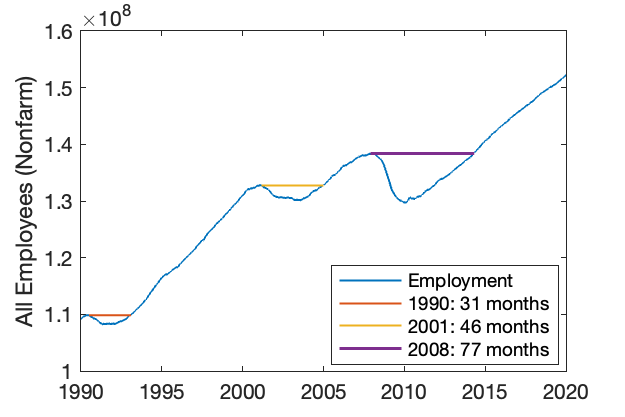
\includegraphics[width=0.48\textwidth]{Employment}
\caption{Employment}
{\small Data source: FRED} 
\label{Employment}
\end{figure}

As shown in figure \ref{UR_LFPR}, after peaking at 10\% in October 2009 (almost 40\% are long-term unemployed), the unemployment rate remained above its pre-recession level until November 2016. Right before the pandemic, the unemployment rate had recovered, and in fact, reached 3.5\% in February 2020, which is the lowest level since 1969. However, the Labor Force Participation Rate (LFPR) remained at a much lower rate (63.3\% in February 2020) than the pre-recession level (66\% in November 2007). \\

\begin{figure}[h!]
\centering
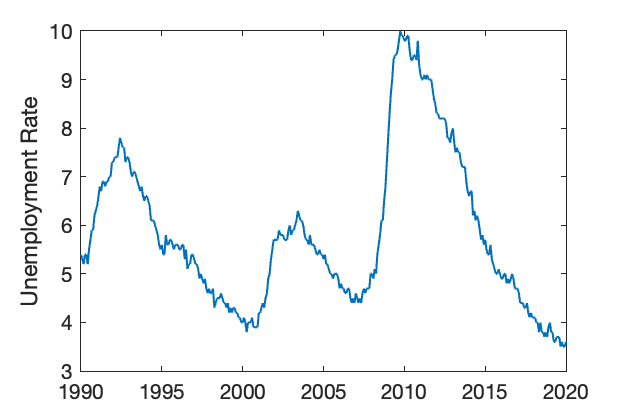
\includegraphics[width=0.48\textwidth]{UR}
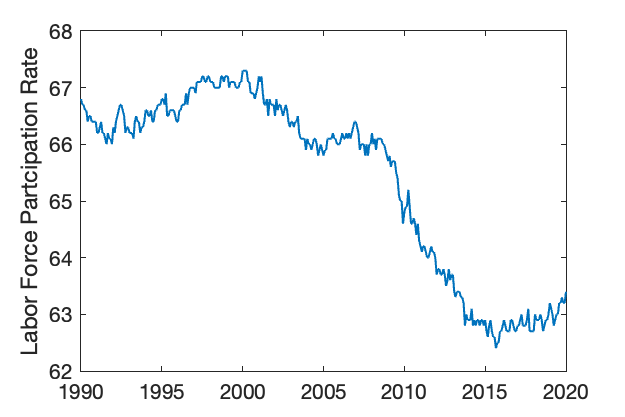
\includegraphics[width=0.48\textwidth]{LFPR}
\caption{Unemployment rate and Labor force participation rate}
{\small Data source: FRED} 
\label{UR_LFPR}
\end{figure}

\subsection{Group heterogeneity}
There was substantial heterogeneity in employment recovery paths across education groups in the 2001 and 2008 recession. As shown in figure \ref{Employment_Education}, the employment of low-skill workers (high school or less) dropped significantly during the Great Recession and much steeper than in the 2001 recession. Also, unlike the quick recovery in the 2001 recession, the employment of low-skilled workers stayed significantly below its pre-recession level after the 2008 recession. In terms of the high skilled workers (some college, bachelor's, and higher), the effect of both recessions on employment was limited, and the recoveries were rapid.  
\begin{figure}[h!]
\centering
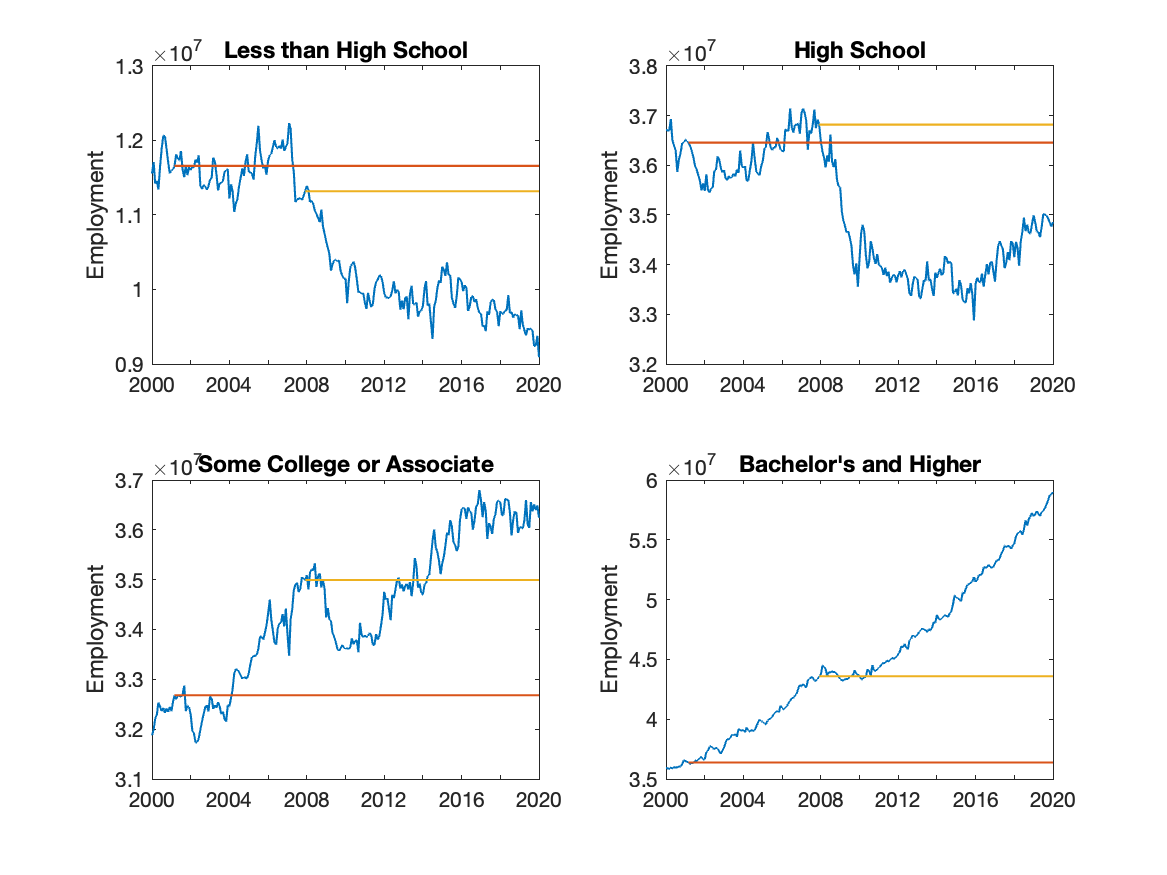
\includegraphics[width=\textwidth]{Employment_Education}
\caption{Employment by Education}
\label{Employment_Education}
\end{figure}


\subsection{State level evidence}
Based on the theoretical prediction of the model, the unemployment can be decomposed into the frictional unemployment $\tilde{u}$ plus the mismatch unemployment $M$ .  
\begin{align*}
u_{it} &= \tilde{u}_{it}+M_{it} 
\end{align*}
Frictional unemployment $\tilde{u}$ is related to the value of vacancy and decreases in skill $H$ and technology $Q$ level. Mismatch unemployment $M$ is related to the probability of unsuccessful matches and increases in the skill-technology difference $|\frac{Q_{it}}{H_{it}}-1|$. Unemployment volatility decreases also in skill $H$ and technology $Q$ level, and increases in skill-technology difference $|\frac{Q_{it}}{H_{it}}-1|$. \\

I employ annual US data from 2007 to 2015; the data was obtained from FRED except for the technology data. I obtain the number of utility patents from the United States Patent and Trademark Office (USPTO), Research and Development (R\&D) investment and the number of Science and Engineering (S\&E) occupations from the National Science Foundation (NSF). Skill is measured by the ratio of the labor force who have bachelor degree; technology is measured by (1) Number of Utility Patent Grants, (2) Ratio between Science and Engineering (S\&E) occupations and all occupations, (3) Ratio between state R\&D investment and state GDP. The measure is computed as the state level deviation from the national mean to make the two measures comparable.
\begin{align*}
\tilde{b}_{it} = \frac{b_{it}-\mean(b_{it})}{\var(b_{it})}
\end{align*}

I use the following regression to test the prediction of the model. I'm interested in the effect of skill level $H$, technology level $Q$ and skill-technology difference $|\frac{Q_{it}}{H_{it}}-1|$ on the state unemployment rate $u$, while I control the state average labor productivity $ALP$, national unemployment rate $\bar{u}$ and the state fixed effect $\alpha_i$. I am also interested in their impact on the unemployment volatility $var$. 
\begin{align*}
u_{it} &= \beta_0+\beta_1Q_{it} +\beta_2 H_{it}+ \beta_3M_{it} +\beta_4 ALP_{it} +\beta_5\bar{u}_t+\alpha_i+\epsilon_{it} \\
var_{i} &= \gamma_0+\gamma_1\overline{Q}_{i} +\gamma_2 \overline{H}_{i}+ \gamma_3\overline{M}_{i} +\gamma_4 \overline{ALP}_{i} +\xi_{i}  \\
M_{it} &= |\frac{Q_{it}}{H_{it}}-1| 
\end{align*}

The regression result is presented in table \ref{unemployment}, technology level is measure by the number of utility patents granted in that state. Consistent with the model's prediction, the unemployment level and volatility are decreasing in skill and technology level but increasing in the skill-technology difference (mismatch level).

\begin{table}[h!]
\centering
\caption{Mismatch unemployment}
\label{unemployment}
\begin{tabular}{lcc} \hline \hline
 & (1) & (2) \\
VARIABLES & Unemployment rate & Unemployment volatility \\ \hline
 &  &  \\
Skill & -9.069*** & -1.712** \\
 & (1.277) & (0.686) \\
Technology & -1.811 & 0.660 \\
 & (1.318) & (0.603) \\
National unemployment rate & 0.870*** &  \\
 & (0.00537) &  \\
Productivity & -1.432*** & 0.557 \\
 & (0.504) & (0.675) \\
Mismatch & 4.589*** & 1.728** \\
 & (0.879) & (0.823) \\
Constant & 12.12*** & 2.044** \\
 & (2.021) & (0.954) \\
 &  &  \\
Observations & 5,400 & 50 \\
R-squared & 0.832 & 0.240 \\
 Number of State & 50 &  \\ \hline
\multicolumn{3}{c}{ Standard errors in parentheses} \\
\multicolumn{3}{c}{ *** p$<$0.01, ** p$<$0.05, * p$<$0.1} \\
\end{tabular}
\end{table}

\clearpage
\section{Conclusion}
The mismatch between the skill and technology level increases the unemployment level and volatility by affecting the expected vacancy value and the probability of matching success. By calibrating the full model to match the data in 1980-1986 and 2007-2013 respectively, I find that the slow jobless recovery after the Great Recession is related to a higher mismatch level. The higher mismatch level is mainly attributed to a higher complementarity between skill and technology, higher skill variance, and lower technology adoption cost. Higher unemployment insurance can decrease the inefficiency caused by mismatch, fewer vacancies are created, and workers only accept better matches. Subsidies to training can decrease the mismatch; workers increase their investment in their training. 

\clearpage
\bibliographystyle{plain}
\bibliography{Mismatch}

\end{document}
